The form of the function $f_\theta$ in~\eqref{eq:learning}
is critical in determining both
the types of optimization methods
that may identify a solution,
and the particular minimizer identified.
In the learning methods that follow,
$f$ will typically take the form of 
a deep neural network.
The advantages
and successes of deep neural networks
rely heavily on their ease of optimization:
the \textit{computation graph} that 
underlies the neural network
allows for gradients
to be computed by parts
and accumulated via the chain rule.

Consider a simple function $f_\theta(x)$
that is defined as a linear combination of 
some parameters $\theta:=w, w\in \RR^d$ with $x\in \RR^d$ followed by 
a differentiable, nonlinear scalar \textit{activation} function $a(\cdot)$:
\begin{align}\label{eq:wx}
	f_\theta(x) := a(w\cdot x)
\end{align}
If we have some estimate of the parameters $\theta:=w$,
then the gradient of the full network with respect to those parameters is
\begin{align}
	\frac{df}{d\theta} = \frac{df}{da}\frac{da}{dw}
\end{align}
where $df/da$ is the (known) derivative of the \textit{activation} function,
and $da/dw$ is exactly $x$, the derivative of a linear function.
With a direction of descent,
we can update the parameters via some update to minimize the functional $f$ of interest:
\begin{align}\label{eq:fullgd}
	\theta_{t+1} = \theta_t + g(\theta_t,x)
\end{align}
where $g(\cdot)$ is some function of the full derivative $g(\cdot) := g(\nabla f_\theta(x))$,
and $\theta_t$ are the current parameter estimates.
Optimization proceeds and terminates when a certain amount
of iterations $t$ have completed,
or some stopping criterion has been reached,
typically that the gradient is small,
indicating that a minima has been identified.

In data science and machine learning applications,
we typically do not have a fixed $x$, but 
rather a dataset $X:=\{x_i\}_{i=1}^n$.
If the dataset is small,
we may be able to still compute an update as in~\eqref{eq:fullgd}.
But this is infeasible when we have thousands,
hundreds of thousands, or millions of samples.
In this case,
stochastic gradient descent (SGD) is used.
Gradient updates in SGD proceed
by taking a single sample and computing~\eqref{eq:fullgd}.
\textit{Training} of $\theta$
follows by iteratively updating the parameters
over full passes of the dataset.
When feasible, mini-batches of samples can
be used instead of a single sample,
and in both cases convergence and convergence
rates have been shown to be reasonable~\citep{hardt2016train}.

\paragraph{Hessians.}
Uninformed gradient updates
are generally preferred
for their speed and ease of computation.
However, additional information in the form of the \textit{Hessian}
can lead to faster convergence
as well as a number of theoretical properties and guarantees.
Consider the function at a critical point $\theta^*$.
The Taylor expansion of the function at that point is
\begin{align}
f(\theta) = f(\theta^*) + \nabla f(\theta^*)^\top f(\theta - \theta^*) + \frac{1}{2}(\theta - \theta^*)^\top H(\theta^*)(\theta - \theta^*) + \ldots
\end{align}
Where $H(\theta^*)$ is the Hessian matrix at the point $\theta^*$. 
With no additional terms, this second-order approximation provides information
about the local curvature of the function near the critical point,
allowing a scaling of the gradient that can use this local 
curvature to inform optimization:
\begin{align}\label{eq:newtonstep}
	\theta_{t+1} = \theta_t + H(\theta_t)^{-1} g(\theta_t)
\end{align}
These Newton updates are typically infeasible in most
machine learning applications with high-dimensional
parameter spaces, where the complexity of
the actual function or the maximal moment is unknown.
In some cases, Hessian approximations,
or its eigenspectrum can be efficiently computed,
and as we will see this can lead to 
practical measures that lead to new
algorithms and guarantees.

For more on these ideas, 
and a formal treatment with respect to 
general optimization, see~\cite{wright1999numerical}.

These formulations and SGD updates generalize
to extremely large and complex stacks
of operations, and are what have enabled
the enormous success and ubiquity of learning
methods.
While ``fully-connected" layers, such as
in~\eqref{eq:wx} are the simple in their form,
they have been proven to be sufficient
in large capacity to serve as
\textit{universal function approximators}~\citep{cybenko1989approximation}.
In this form however, capacity guarantees
require the number of parameters (dimension of $w$)
to grow exponentially: infeasible in practice.
If the size is misspecified, training
can lead to parameter settings that are provably
optima at that level, but fail to sufficiently
capture the true problem complexity.
These problems extend to stacks of ``fully-connected"
layers as well: nonlinearity through multiplication
and activations is effective, but leads
to poor training time results due to 
the speed at which a local minima can be found.\todo{whats the citation here}

The final minima identified 
can vary significantly based on 
the particular form of the function $f_\theta$, 
and, in the case where the function $f$ is not \textit{convex}, 
it can also depend on the estimate $\theta_0$ at initialization.
This detail has been used to suggest
that large, complex neural networks 
may contain sub-networks that can be trained in isolation
to perform a task with high accuracy,
even when randomly initialized.
The ``lottery ticket hypothesis" states 
a small, sparse sub-network can be trained to perform just as well as the larger network, 
but with fewer parameters and less computation.
\begin{figure}
	\centering
	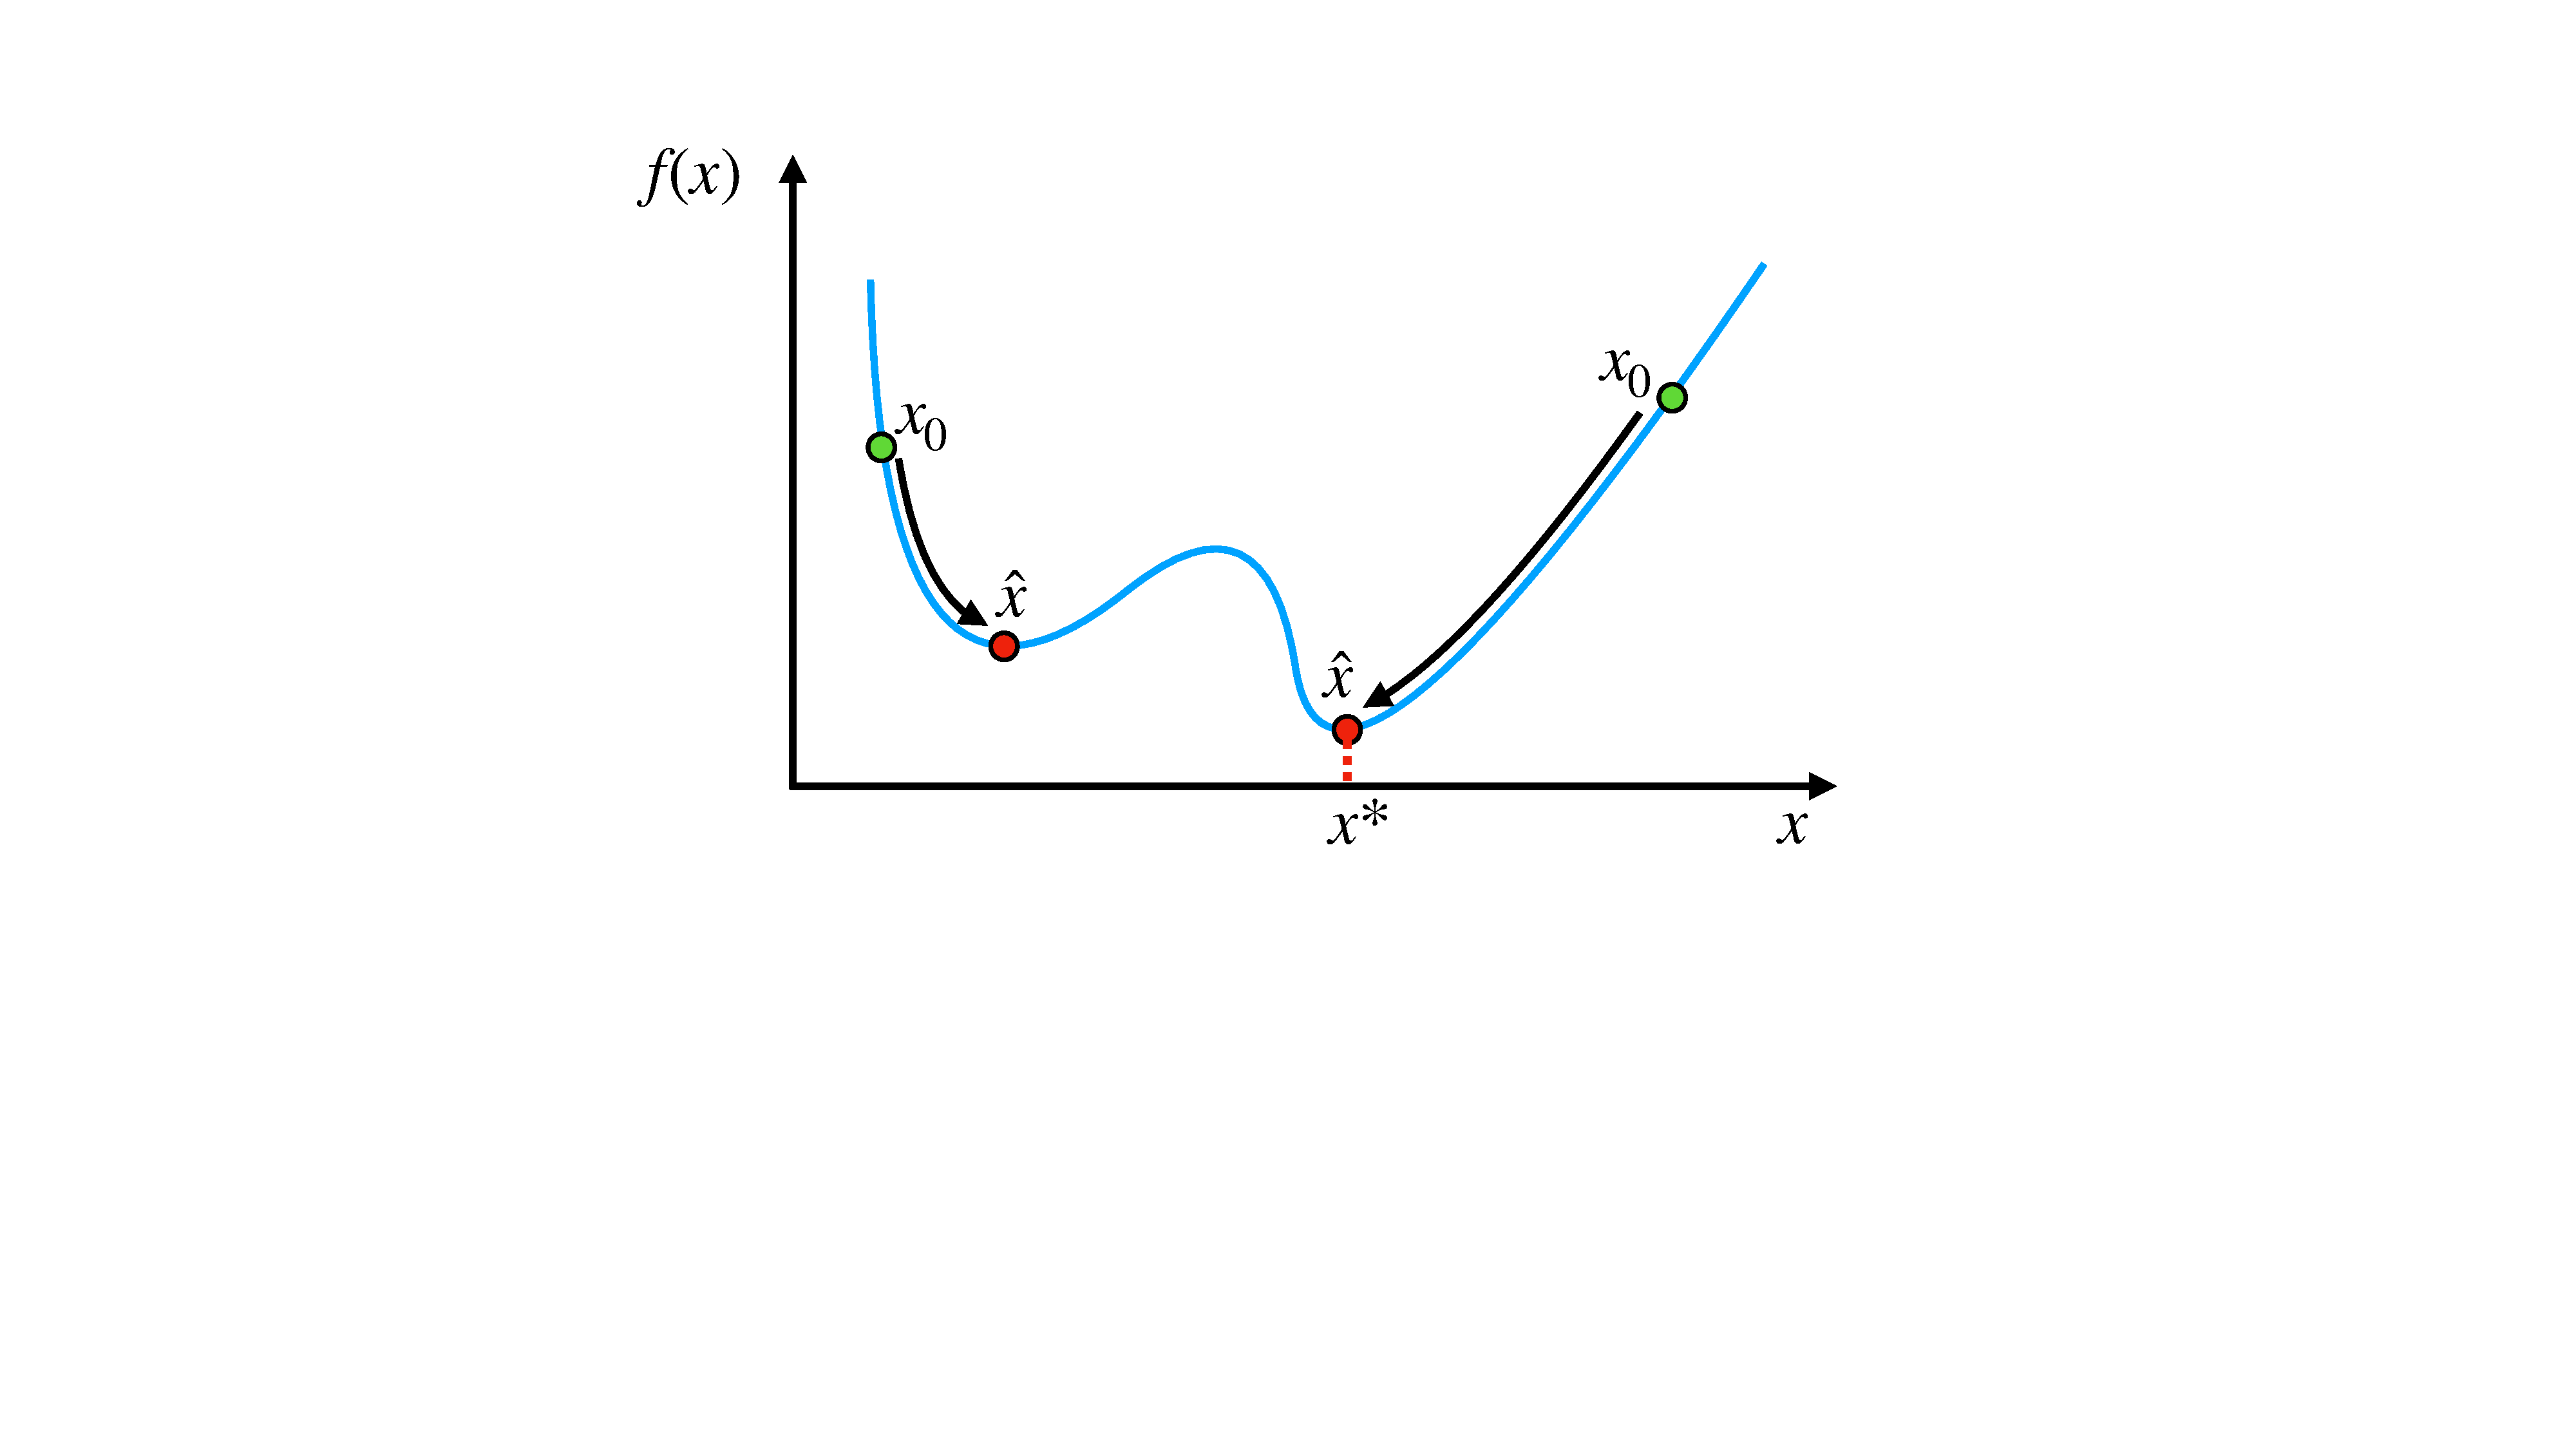
\includegraphics[width=0.75\textwidth,trim={15cm 15cm 15cm 1cm},clip]{2_bknd/localmin.pdf}
	\caption[Importance of initialization in nonconvex problems]{Nonconvex functions $f(x)$ optimized using variations of gradient descent can lead to different (and potentially non-global) optima ($\hat{x}$).}
	\label{fig:localmin}
\end{figure}

A wide variety of neural network \textit{architectures}
have been proposed depending on the type of data and learning task.
Some of the most commonly used architectures include
Convolutional Neural Networks (CNNs), Recurrent Neural Networks (RNNs),
Transformers, Autoencoders, and Generative Adversarial Networks (GANs).
CNNs, mainly used in image recognition and processing tasks,
use convolutions designed to process grid-like imaging data. 
RNNs are designed to handle sequential data such as time series or language,
and have a memory-like mechanism that allows information to persist in hidden state vectors. 
Transformers, now the de-facto method in Natural Language Processing (NLP),
make use of a self-attention mechanism,
weighing the importance of different input tokens for eventual prediction~\citep{vaswani2017attention}. 
Autoencoders and Generative Adversarial Networks (GANs) fall under the category of generative models,
trained to generate outputs that resembles real data. 
Newer generative models built on diffusion methods have 
been able to produce photorealistic images based
only on captions input by the user~\citep{rombach2022high}.
All of these methods come with their own
idiosyncracies in model capacity and practical
methods for efficient training~\citep{lecun2015deep}.

With these varying architectures
has also come the field of \textit{architecture search},
identifying the hyperparameters and layer types
that would lead to the best downstream performance
with the most efficient full architecture.
While computationally expensive, techniques
such as reinforcement learning, evolutionary algorithms,
gradient-based methods, and even greedy approaches
have been used to identify state-of-the-art networks~\citep{elsken2019neural}.

\subsection{Losses and Probability Measures}
The methods for optimization above
lend themselves to typically arbitrary functions.
As described in the Introduction,
typically a \textit{loss function}
is defined to measure the disparity
between the prediction or output of a model
and the target of interest.
Optimizer flexibility has led
to the development and design of loss functions
that suit particular tasks,
or those that correspond more directly
to practitioners' high-level goals.
Building on the classical mean-squared error,
$l(f_\theta(x), y) := (y - f_\theta(x))^2$,
methods have extended to information-based schemes
such as cross-entropy, as well as 
incorporating classical \textit{regularization} schemes
to push solutions towards desirable minima.
These typically take the form of additive terms 
penalizing large norms over weights, where
the norm chosen corresponds to the choice of 
prior assumed by the user.

Following the information-based schema,
significant work has been done
on probabilistic forms of losses,
treating the input and output spaces
of models as distributions.
Particularly useful for generative models,
$f$-divergences have been studied
as a general form of distances
between probability distributions
that can be effectively minimized to
train in such a way that model outputs
come from a maximum-entropy distribution
with respect to the original training data~\citep{fgan}.
Measures such as KL-divergence, mutual information,
maximum-mean discrepency, and others all fall within
this framing.

\subsection{Optimal Transport}	
Of particular interest in this thesis is the \textit{Wasserstein} distance,
or traditionally known as the Earth Mover's distance.
Recent developments in GANs \citep{wgan} have demonstrated
the Wasserstein metric is typically more stable
compared to other measures and avoids
\textit{mode collapse}, sharp local minima 
with low variation. Interestingly
this formulation can be viewed as an approximation
of the \textit{optimal transport} problem.

Optimal transport refers to the problem of finding
a transportation plan that minimizes some cost of transforming
one probability distribution to another.
Developments in Riemannaian geometry and measure theory 
have led to a general formulation.
\begin{definition}[Monge-Kantorovich Problem \citep{kantorovich}]\label{def:mongekant}
	Let $\mu,\nu$ be probability measures over separable metric spaces $X$ and $Y$.
	The optimal transportation problem seeks to find a joint measure $\gamma$ on $X\times Y$
	that satsifies
	\begin{align}
	\gamma^* = \text{inf} \left\{\left. \int_{X\times Y} c(x,y) d\gamma(x,y) \right| \gamma \in \Gamma(\mu,\nu) \right\}
	\end{align}
\end{definition}
Where $\Gamma$ is the space of all probability measures with marginals equal to $\mu$ on $X$ and $\nu$ on $Y$.
More common in recent machine learning is the \textit{Wasserstein} distance,
defined as the $p$-th distance over the Monge-Kantorovich problem.
\begin{definition}[Wasserstein metric]\label{def:wassmetric}
	The Wasserstein $p$-distance is given by:
	\begin{align}
	W_p(\mu, \nu) = \left( \inf_{\gamma \in \Gamma(\mu, \nu)} \EE_{(x, y) \sim \gamma} d(x, y)^p \right)^{1/p}
	\end{align}
\end{definition}
And the discrete analog:
\begin{definition}[Earth Mover's Distance]
	Let $p_1$ and $p_2$ be distributions with discrete support of size $n$, and $x(i,j)$, where  $x\in\RR^{n\times n}$, denotes the movement of ``mass" from $p_1(i)$ to $p_2(j)$.
	Denote by $c(i,j)$ the cost of moving one unit of mass from  $p_1(i)$ to $p_2(j)$.
	The Earth Mover's Distance (EMD) between $p_1$ and $p_2$ is the minimal cost to transform $p_1$ into $p_2$.
	%given by the sum of the costs associated with shifting mass, according to $x(i,j)$ such that $p_1$ is transformed into $p_2$.
	% Unless otherwise specified, we assume $c(i,j)=|i-j|$, which corresponds to ground distance. 
	%This can be 
	Written as a linear program (LP):
	\begin{align}\label{eq:2d-emd}
	\begin{aligned}
	\underset{{x\in \RR^{n\times n}_+}}{\textrm{min}} \sum_{i,j} c(i,j) x(i,j) \quad  \textrm{s.t.}\quad \sum_j x(i,j) &= p_1(i); \ 
	\sum_i x(i,j) = p_2(j),\ (\forall i,j\in[n]).
	\end{aligned}
	\end{align}
\end{definition}
\begin{figure}
	\centering
	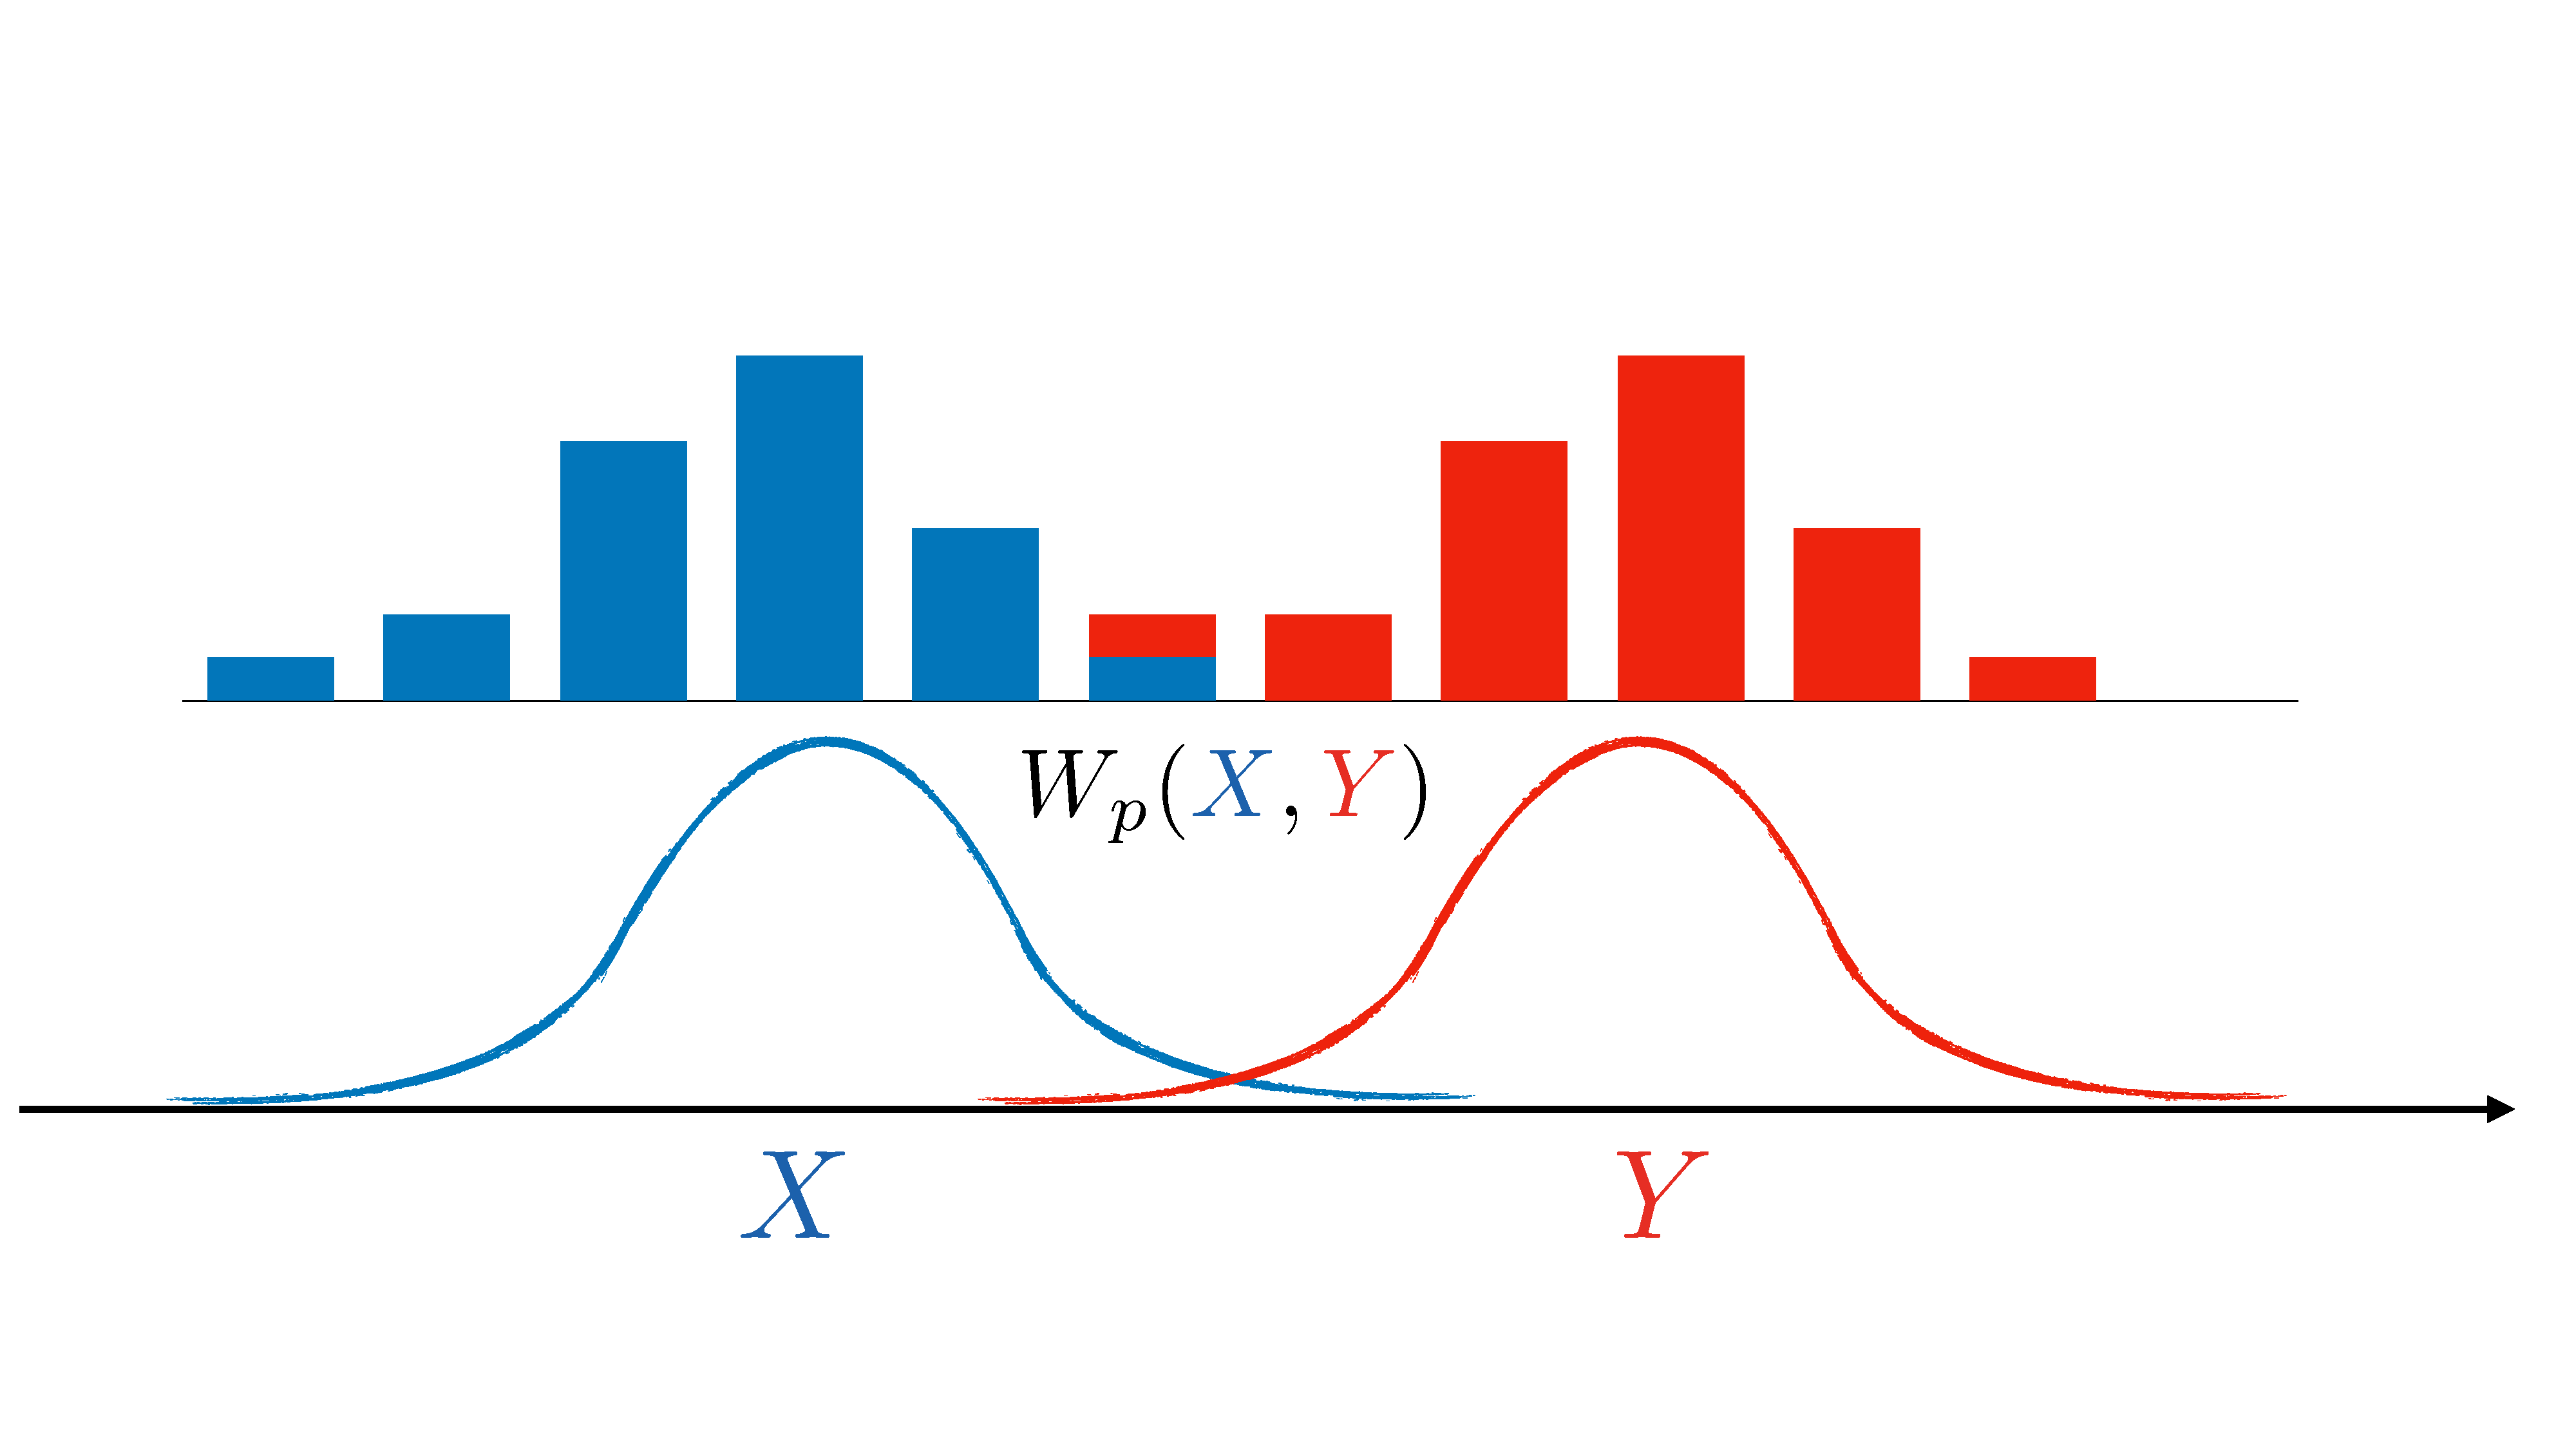
\includegraphics[width=\textwidth,trim={0 5cm 0 10cm},clip]{2_bknd/ot.pdf}
	\caption[Distributions and Optimal Transport]{2D Optimal transport measures the distance or cost associated with transforming one discrete or continuous distribution to another.}
	\label{fig:bkndot}
\end{figure}
Computation of the continuous measures can be straightforward with some assumptions,
leading to natural linear programming formulations akin to the EMD.
However in cases where one wishes to \textit{minimize} this distance,
practical complexity explodes, even in the discrete
formulations commonly found in application.
A new entropic regularization method introduced in \cite{cuturi2013sinkhorn}
has led to newfound interest,
use, and analysis of optimal transport for deep learning applications.
In Chapter~\ref{chap:demd} we will expand upon these
ideas to the case where we have multiple distributions,
and wish to minimize the distance among all of them concurrently.
